\documentclass[12pt]{report}

\usepackage{geometry}
\geometry{a4paper,scale=0.8}

\usepackage{indentfirst}
\usepackage{caption}
\usepackage{graphicx, subfig}

\usepackage[BoldFont,SlantFont,CJKchecksingle]{xeCJK}
\setCJKmainfont[BoldFont=SimHei,SlantedFont=KaiTi]{SimSun}
\setCJKsansfont[BoldFont=SimHei,SlantedFont=KaiTi]{SimSun}
\setCJKmonofont[ItalicFont={Adobe Fangsong Std}]{SimSun}
\setCJKfamilyfont{zhsong}{SimSun}
\setCJKfamilyfont{zhhei}{SimHei}
\setCJKfamilyfont{zhkai}{KaiTi}
\setCJKfamilyfont{zhfs}{FangSong}

	
\title{社交网络}
	
\author{高一鸣 21721126}

\date{}

\begin{document}
		
	\maketitle
		
	\tableofcontents
	
	\renewcommand\thesection{\arabic {section}}
		
	\section{社交网络介绍}
	
		社交网络是由许多节点构成的一种社会结构。节点通常是指个人或组织,而社交网络代表着各种社会关系。
			
		这个名词是1954年由J. A. Barnes 首先使用 ("Human Relations" , 在章节 Class and Committees in a Norwegian Island Parish 内)。一个社交网络的大小最大约为150人左右 (Dunbar's number),平均大小约为124人左右 (Hill and Dunbar, 2002)。
		
		社交网络源自网络社交,网络社交的起点是电子邮件。互联网本质上就是计算机之间的联网,早期的E-mail解决了远程的邮件传输的问题,至今它也是互联网上最普及的应用,同时它也是网络社交的起点。
		
		BBS则更进了一步,把“群发”和“转发”常态化,理论上实现了向所有人发布信息并讨论话题的功能(疆界是BBS的访问者数量)。BBS把网络社交推进了一步,从单纯的点对点交流的成本降低,推进到了点对面交流成本的降低。
		
		即时通信(IM)和博客(Blog)更像是前面两个社交工具的升级版本,前者提高了即时效果(传输速度)和同时交流能力(并行处理);后者则开始体现社会学和心理学的理论——信息发布节点开始体现越来越强的个体意识,因为在时间维度上的分散信息开始可以被聚合,进而成为信息发布节点的“形象”和“性格”。比如从RSS、flickr到最近的YouTube、Digg、Mini-feed、Twitter、Fetion、Video-Mail都解决或改进了单一功能,是丰富网络社交的工具。
		
		随着网络社交的悄悄演进,一个人在网络上的形象更加趋于完整,这时候社交网络出现了。交友只是社交网络的一个开端,就像Google的开端只是每个网页的backlinks那么普通一样,社交网络的开端只是获取你的个人资料和好友列表。
		
		社交网络大体经历了这样一个发展过程:
		\begin{itemize}
			\item 早期概念化阶段──SixDegrees代表的六度分隔理论
			\item 结交陌生人阶段──Friendster帮你建立弱关系从而带来更高社会资本的理论
			\item 娱乐化阶段──MySpace创造的丰富的多媒体个性化空间吸引注意力的理论
			\item 社交图阶段──Facebook复制线下真实人际网络来到线上低成本管理的理论
			\item 云社交阶段——著云台分布式网际社交理论
		\end{itemize}
		
		整个SNS发展的过程是循着人们逐渐将线下生活的更完整的信息流转移到线上进行低成本管理,这让虚拟社交越来越与现实世界的社交出现交叉。
		
		人类历史上,大凡重要的技术革命都伴随媒介革命,人类任何活动本质上都是信息活动,信息流的传递介质、管理方式的不同将决定你接受信息的不同,所有有关信息流媒介的变革一定是底层的变革——网络社交也是如此。从网络社交的演进历史来看,它一直在遵循“低成本替代”原则。网络社交一直在降低人们社交的时间和物质成本,或者说是降低管理和传递信息的成本。
		
		与此同时,网络社交一直在努力通过不断丰富的手段和工具,来替代传统社交来满足人类这种社交动物的交流需求,并且正在按照从“增量性的娱乐”到“常量性的生活”这条轨迹不断接近基本需求。
		
		如果说在网络社交的起点——电子邮件时代,网络仅仅可以满足人们5\%的社交需求,那么今天丰富的社交网络已经可以把这个数字至少提升了10倍,除了“接触型”的社交行为,或者说是“接触型”信息的收集和发布之外,网络社交已经开始承担大部分传统社交的作用。实际上,“非接触型”的社交,原本就占据了人类社交的80\%以上,这意味着网络社交对传统世界必然会带来巨大的影响。
		
		说到底,网络社交不仅仅是一些新潮的商业模式,从历史维度来看,它更是一个推动互联网向现实世界无限靠近的关键力量。社交网络涵盖以人类社交为核心的所有网络服务形式,互联网是一个能够相互交流,相互沟通,相互参与的互动平台,互联网的发展早已超越了当初ARPANET的军事和技术目的,社交网络使得互联网从研究部门、学校、政府、商业应用平台扩展成一个人类社交的工具。
		
		网络社交更是把其范围拓展到移动手机平台领域,借助手机的普遍性和无线网络的应用,利用各种交友/即时通讯/邮件收发器等软件,使手机成为新的社交网络的载体。社交网络,也就是网络+社交的意思。通过网络这一载体把人们连接起来,从而形成具有某一特点的团体。
		
		但也必须注意到,人与人之间的信息沟通,近7\%的信息通过语言传递的(文字更少),语气、情感、态度、肢体语言等占了93\%。除非网络社交的发展逼近传统接触型社交效果,否则只能是有益的补充,真正认识了解一个人还是需要在现实中接触才行,此段内容有意无意夸大了网络虚拟社交的作用。其实认识了这点也为网络社交指明了外来发展方向(类似星球大战中的远程全息“面对面”交流)。最近研究表明,依赖Facebook进行社交的人易发生抑郁情绪。
	
	\section{社交网络理论}
		
		社交网络主要包含以下几个核心的理论。
	
		\subsection{顿巴数(150定律)}
		
			150定律(Rule Of 150),即著名的“邓巴数字”,由英国牛津大学的人类学家罗宾·邓巴(Robin Dunbar)在20世纪90年代提出。
			
			该定律根据猿猴的智力与社交网络推断出:人类大脑的逻辑和记忆力结构,注定了大脑可以容纳148人的稳定社交关系,四舍五入大约是150人,这就是著名的“顿巴数”。按照顿巴数的规律,一个社会群组合适的规模大约为150人,超过这个数字就无法有效地沟通和协作。
			
			该定律指出:人的大脑新皮层大小有限,提供的认知能力只能使一个人维持与大约150个人的稳定人际关系,这一数字是人们拥有的、与自己有私人关系的朋友数量。也就是说,人们可能拥有150名好友,甚至更多社交网站的“好友”,但只维持与现实生活中大约150个人的“内部圈子”。而“内部圈子”好友在此理论中指一年至少联系一次的人。
			
			根据顿巴教授的研究,人类的社会结构表现为:5人左右的亲密接触圈;12-15人的同情圈,即,如果这一圈里有人去世,我们会很伤心;50人左右的群落,即经常一起生活、一起行动的人(已经有限定在这一人数内的社交网络工具出现);150人左右的氏族,即遵从共同仪式的人;500人左右的部落,即拥有同种语言的人(其实在现代社会,这里的语言有时只是指一些经常交流的人之间约定俗成的词语和概念,外人第一次听到不能理解);5000人左右的群落,即有共同文化的人。按照顿巴数的同心圆模型,当社会结构的人数超过150人时,相互间的互动和影响就会减少很多,只能靠共同的语言来维系,而当人数上升到5000人左右时,维系社会结构则只能依靠共同的文化。”
		
		\subsection{“六度分隔”理论}
		
			1967年,美国哈佛大学的心理学教授Stanley Milgram(1933-1984)想要描绘一个连结人与社区的人际联系网,做过一次连锁信件实验,结果发现了"六度分隔"现象。六度分隔(Six Degrees of Separation)现象(又称为“小世界现象”small world phenomenon),可通俗地阐述为:“你和任何一个陌生人之间所间隔的人不会超过五个,也就是说,最多通过五个人你就能够认识任何一个陌生人。”
			
			其数学解释如下:若每个人平均认识260人,其六度就是260的(6-1)次幂为1,188,137,600,000。消除一些节点重复,那也几乎覆盖了整个地球人口若干多多倍。
			
			Stanley Milgram的实验如下:他从内布拉斯加州和堪萨斯州招募到一批志愿者,随机选择出其中的三百多名,请他们邮寄一个信函。信函的最终目标是米尔格兰姆指定的一名住在波士顿的股票经纪人。由于几乎可以肯定信函不会直接寄到目标,米尔格兰姆就让志愿者把信函发送给他们认为最有可能与目标建立联系的亲友,并要求每一个转寄信函的人都回发一个信件给米尔格兰姆本人。出人意料的是,有六十多封信最终到达了目标股票经济人手中,并且这些信函经过的中间人的数目平均只有5个。也就是说,陌生人之间建立联系的最远距离是6个人。
			
			“六度分隔”理论奠定了社交网络的理论基础,米尔格拉姆的这个连锁实验体现了一个似乎很普遍的客观规律:社会化的现代人类社会成员之间,都可能通过“六度空间”而联系起来,绝对没有联系的A与B是不存在的。
		
		\subsection{贝肯数}
			
			贝肯数(Bacon numbers)是一个“六度分割理论”基础上的概念,是描述好莱坞影视界一个演员与著名影星凯文·贝肯的“合作距离”的一种方式。贝肯是好莱坞的一名普通演员,不同于马龙·白兰度这样的大腕,贝肯在好莱坞电影中从来都是以配角的身份出现,他与当时好莱坞的影视明星发生联系所需要的中间人数量即为“贝肯数”。
			
			弗吉尼亚大学一个实验室曾为约25万上过银幕的男女演员计算了他们的“平均贝肯数”,研究发现无论是历史上贝肯数最低的演员罗德·斯泰格尔还是一个名不见经传的小演员,他们的贝肯数都在2.6和3之间,并且相差十分微小。
			
			这一发现说明,其实你要想进入网络的链接中心,并不一定要成为大人物,你成为一个“永不退场”的配角也可以非常接近网络的中心,你和中心人物的距离其实可以近到忽略不计,因为那不是一个物理距离,而只是一个链接度的问题。
			
			“贝肯数”的发现还说明要想阻断一个网络和另一个网络的链接(比如让马龙·白兰度永远和某个导演无法接触到),隔离“贝肯”这样的高链接性人物就可以了。同样,一个网络社区的崩溃,其实不会因为多少普通用户流失而发生,但几个节点用户的流失,就会造成崩溃。
			
			虽然六度人脉理论将我们大多数人相连,但是总有那些掌握着重要人脉的节点,通过他们,六度空间才能顺利形成通路。
			
		\subsection{强弱关系链}
		
			马克·格拉诺维特在1973年发表的论文指出:在传统社会,每个人接触最频繁的是自己的亲人、同学、朋友、同事等,这是一种十分稳定的然而范围有限的社会关系,这是一种“强关系” ;同时,还存在另外一类相对于前一种社会关系较浅,然而却是更为广泛的社会关系,格兰诺维特把后者称为"弱关系"。
			
			这里将关系强度等级划分与定义:
			\begin{itemize}
				\item 强关系,你基本上每天都能接触或是一个星期至少有2-3次来往的人
				\item 弱关系,不是每天接触的人,但基本上是曾经的朋友,同学,同事,亲戚
				\item 微关系,通过共同的兴趣、爱好、经历形成的泛泛之交
			\end{itemize}
		
			研究发现:其实与一个人的工作和事业关系最密切的社会关系并不是“强关系”,而常常是“弱关系”。“弱关系”虽然不如“强关系”坚固,却有着极快的、可能具有低成本和高效能的传播效率。
			
			弱关系在我们与外界交流时发挥了关键的作用,为了得到新的信息,我们必须充分发挥弱关系的作用。这些弱关系,或是熟人,都是我们与外界沟通的桥梁,不同地方的人通过弱关系可以得到不同的信息。最亲近的朋友可能生活圈子和你差不多,你们的生活几乎完全重合。而那些久不见面的人,他们可能掌握了很多你并不了解的情况。只有这些“微弱关系”的存在,信息才能在不同的圈子中流传。弱关系的威力正在于此。
			
			强连接关系通常表明行动者彼此之间具有高度的互动,在某些存在的互动关系型态上较亲密,因此,透过强关系所产生的讯息通常是重复的,容易自成一个封闭的系统。网络内的成员由于具有相似的态度,高度的互动频率通常会强化原本认知的观点而降低了与其它观点的融合,故认为在组织中强关系网络并不是一个可以提供创新机会的渠道。
			
			事实上,强弱关系并不仅由人与人之间的关系类型决定,还会由六度理论的度数决定。可以理解的是:1度关系肯定要比2度关系强。此外,如果在SNS中,强弱关系还可能会根据建立关系的依据来决定,同好/同兴趣、同群组/同圈子、同应用,这类关系相对较弱,但同一类关系的交集越多关系则可能会越强。
			
			在不同应用场景下,强弱关系链有着明显的差异。在手机同步通信、IM异步通信的场景下,强关系链发挥了主导作用。但是类似微博这类新兴媒体更多的是兴趣导向,信息的爆炸传播,弱关系链更容易突破顿巴数的限制,达到社交圈的快速增长。
			
		\subsection{二八定律(巴莱多定律)}
			
			社交网络中除了有强弱关系链分析,还有重要和不重要之分。二八定律最早是在19世纪末20世纪初由意大利经济学家巴莱多发现提出的,是指二成的人拥有八成的人的财富。
			
			他认为,在任何一组东西中,最重要的只占其中一小部分,约20\%,其余80\%的尽管是多数,却是次要的,因此又称二八定律。
			
			后来,二八定律延伸到各个领域,包括人脉,例如20\%的人脉给你带来80\%的价值。
			
		\subsection{马太效应}
				
			1968年,美国科学史研究者罗伯特·莫顿(Robert K. Merton)提出这个术语用以概括一种社会心理现象:“相对于那些不知名的研究者,声名显赫的科学家通常得到更多的声望;即使他们的成就是相似的,同样地,在一个项目上,声誉通常给予那些已经出名的研究者”。马太效应反映的社会现象是两极分化,富的更富,穷的更穷。
			
			罗伯特·莫顿归纳“马太效应”为:任何个体、群体或地区,在某一个方面(如金钱、名誉、地位等)获得成功和进步,就会产生一种积累优势,就会有更多的机会取得更大的成功和进步。
			
			马太效应揭示了一个大概率事件:社交网络中重要的节点很可能会越来越重要,而位于网络边缘的节点,可能会越来越被弱化。社会交往中,那些长于交际朋友多的人会借助频繁的交往,认识更多的朋友;那些内向沉默的人则会越来越孤独。马太效应是个悖论,在受欢迎的社交网络中作为强者的节点泄露隐私的风险越大。
			
		\subsection{长尾效应}
		
			2004年10月,美国《连线》杂志主编克里斯·安德森(ChrisAnderson)在他的文章中第一次提出长尾(Long Tail)理论,他告诉读者:商业和文化的未来不在热门产品,不在传统需求曲线的头部,而在于需求曲线中那条无穷长的尾巴。
			
			“头”(head)和“尾”(tail)是两个统计学名词。正态曲线中间的突起部分叫“头”;两边相对平缓的部分叫“尾”。从人们需求的角度来看,大多数的需求会集中在头部,而这部分我们可以称之为流行,而分布在尾部的需求是个性化的,零散的小量的需求。而这部分差异化的、少量的需求会在需求曲线上面形成一条长长的“尾巴”,而所谓长尾效应就在于它的数量上,将所有非流行的市场累加起来就会形成一个比流行市场还大的市场。
			
			对于社交网络来说,并不是八成不重要的节点就没有用。虽然社交网络中存在不太重要的节点,但是对于一个覆盖面很广的社交网络来说,八成重要性并不是最重要的节点也有其商业开发的价值,互联网的浪潮已经将商品成本降至极低,长尾理论将发挥巨大的价值。
			
		\subsection{羊群效应}
		
			“羊群效应”也叫“从众效应”:是个人的观念或行为由于真实的或想象的群体的影响或压力,而向与多数人相一致的方向变化的现象。表现为对特定的或临时的情境中的优势观念和行为方式的采纳(随潮)表现为对长期性的占优势地位的观念和行为方式的接受(顺应风俗习惯)。人们会追随大众所同意的,将自己的意见默认否定,且不会主观上思考事件的意义。
			
			古斯塔夫·勒·邦(Gustave Le Bon)认为一个心理群体表现出的最显著的特点是:无论构成这个群体的个人是谁,他们的生活方式、职业、性格、智力有多么的相似或者不相似,只要他们构成了一个群体,他们的感觉、思考、行为方式就会和他们处于独立状态时有很大的不同.
			
			社交网络中的节点都会互相影响,每个个体都会偏向大多数人的判断,每个个体都有从众的趋向性。
			
		\subsection{马斯洛需求模型}
		
			马斯洛需求层次理论是人本主义科学的理论之一,由美国心理学家亚伯拉罕·马斯洛在1943年在《人类激励理论》论文中所提出。书中将人类需求像阶梯一样从低到高按层次分为五种,分别是:生理需求、安全需求、社交需求、尊重需求和自我实现需求。
			
			五种需要像阶梯一样从低到高,按层次逐级递升,但这样次序不是完全固定的,可以变化,也有种种例外情况。需求层次理论有两个基本出发点,一是人人都有需要,某层需要获得满足后,另一层需要才出现;二是在多种需要未获满足前,首先满足迫切需要;该需要满足后,后面的需要才显示出其激励作用。一般来说,某一层次的需要相对满足了,就会向高一层次发展,追求更高一层次的需要就成为驱使行为的动力。相应的,获得基本满足的需要就不再是一股激励力量。
			
			五种需要可以分为两级,其中生理上的需要、安全上的需要和感情上的需要都属于低一级的需要,这些需要通过外部条件就可以满足;而尊重的需要和自我实现的需要是高级需要,他们是通过内部因素才能满足的,而且一个人对尊重和自我实现的需要是无止境的。同一时期,一个人可能有几种需要,但每一时期总有一种需要占支配地位,对行为起决定作用。任何一种需要都不会因为更高层次需要的发展而消失。各层次的需要相互依赖和重叠,高层次的需要发展后,低层次的需要仍然存在,只是对行为影响的程度大大减小。
			
			马斯洛和其他的行为心理学家都认为,一个国家多数人的需要层次结构,是同这个国家的经济发展水平、科技发展水平、文化和人民受教育的程度直接相关的。在发展中国家,生理需要和安全需要占主导的人数比例较大,而高级需要占主导的人数比例较小;在发达国家,则刚好相反。
			
			社交网络中的节点是千差万别的,节点间的联系是多种多样的,但归根结底,社交网络是因为满足每个个体的需求而存在,并基于需求模型而发展演变。
			
	\section{社交网络分析}
			
		社交网络分析是一种基于信息学、数学、社会学、管理学和心理学等科学的交叉科学。根据社交网络的特性,其主要研究三大内容:结构与演化,群体与互动,信息与传播。
		
		\begin{figure}
			\centering
			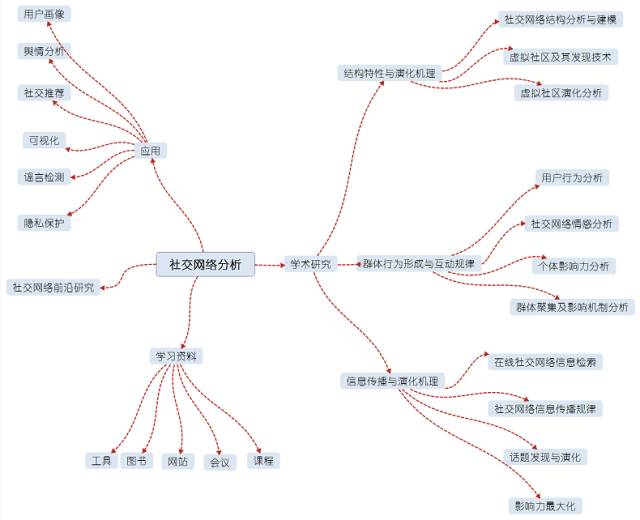
\includegraphics[width=0.8\textwidth]{img/SNA.jpg}
			\caption{社交网络分析结构图} 
			\label{img}
		\end{figure}
		
		\subsection{结构特性与演化机理}
		
			\subsubsection{基本要素}
			
				社交网络模型许多概念来自于图论,因为社交网络模型本质上是一个由节点(人)和边(社交关系)组成的图。主要包括以下要素:
				
				\begin{itemize}
					\item 节点(Node):节点是指要分析的物体,每一个物体就是一个节点,比如在Social Network中每个人就是一个节点。
					\item 边(Edge):Graph中两个节点间的连线,用于表示两个节点的关系。比如在Social Network中两个人的关注关系,微博传播中转发关系。
					\item 图是用来表示一组物体之间的关系的方式。有向图(Directed Graph):边代表的关系具有方向的图。比如微博的关注关系,电话拨入呼出,银行转账收账就是有方向的。无向图(Undirected Graph):边代表的关系没有方向的图。
					\item 度(Degree):节点的度是指与其相连的边数,你通讯录的名单长度就是你的联络人度数。网络平均度反应了网络的疏密程度,而通过度分布则可以刻画不同节点的重要性。
					\item 输入度(In-degree):有向图中一个节点收到的边。
					\item 输出度(Out-degree):有向图中一个节点发出的边。
					\item 路径(Route): 两个节点之间经过的边和节点序列,路径有长度,通常衡量两个点之间的距离。
					\item 网络密度(Density):网络密度可以用于刻画节点间相互连边的密集程度,定义为网络中实际存在边数与可容纳边数上限的比值,常用来测量社交网络中社交关系的密集程度及演化趋势。
					\item 聚类系数(Clustering Coefficient):用于描述网络中与同一节点相连的节点间也互为相邻节点的程度。其用于刻画社交网络中一个人朋友们之间也互相是朋友的概率,反应了社交网络中的聚集性。
					\item 介数(Betweeness):为图中某节点承载整个图所有最短路径的数量,通常用来评价节点的重要程度,比如在连接不同社群之间的中介节点的介数相对于其他节点来说会非常大,也体现了其在社交网络信息传递中的重要程度。
				\end{itemize}
			
			\subsubsection{网络特性}
			
				小世界现象:小世界现象是指地理位置相距遥远的人可能具有较短的社会关系间隔。小世界现象在在线社交网络中得到了很好地验证,根据2011年 Facebook 数据分析小组的报告, Facebook 约7.2亿用户中任意两个用户间的平均路径长度仅为4.74,而这一指标在推特中为4.67。可以说,在五步之内,任何两个网络上的个体都可以互相连接。
				
				无标度特性:大多数真实的大规模社交网络都存在着大多数节点有少量边,少数节点有大量边的特点,其网络缺乏一个统一的衡量尺度而呈现出异质性,我们将这种节点度分布不存在有限衡量分布范围的性质称为无标度。无标度网络表现出来的度分布特征为幂律分布,这就是此类网络的无标度特性。
			
			\subsubsection{网络模型}
				
				规则图:有n个节点,每个节点有d个邻居节点,每个节点只和邻居节点相连。
				
				\begin{figure}
					\centering
					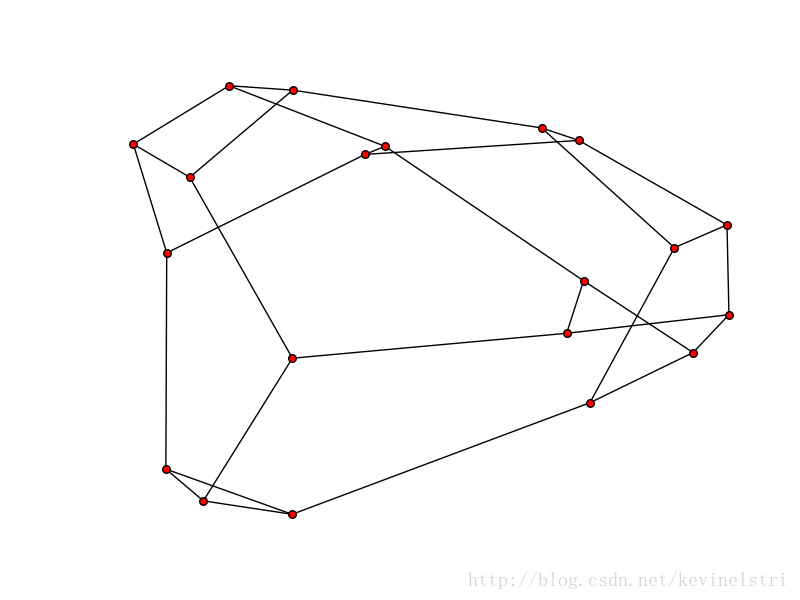
\includegraphics[width=0.6\textwidth]{img/regular.png}
					\caption{规则图} 
					\label{img}
				\end{figure}
				
				ER随机图:有n个节点,每个节点以概率p连接n个节点。
				
				\begin{figure}
					\centering
					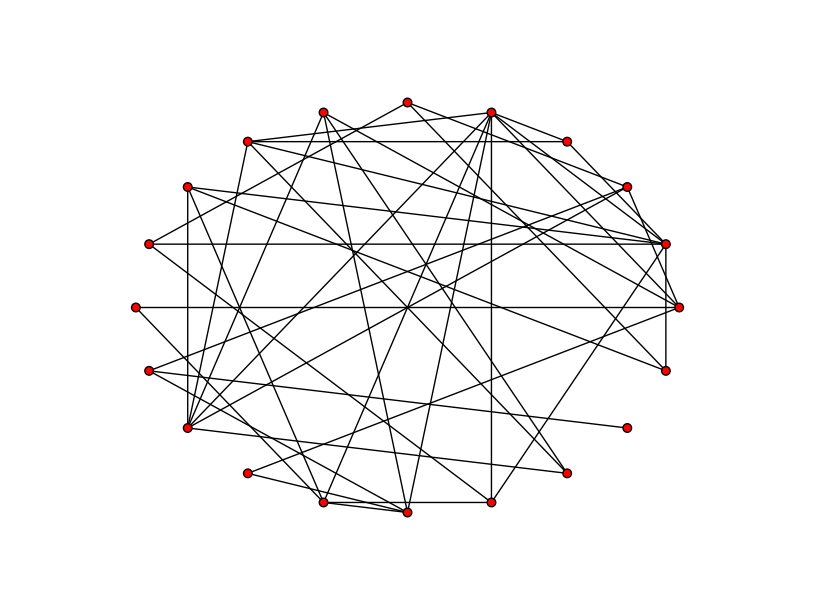
\includegraphics[width=0.6\textwidth]{img/ER.png}
					\caption{ER随机图} 
					\label{img}
				\end{figure}
				
				WS模型:有n个节点,每个节点有k个邻居,每个节点先和周围的邻居节点相连,然后以概率p随机地重新连接网络中的每个边,即将边的一个端点保持不变,而另一个端点取为网络中随机选择的一个节点(其中规定,任意两个不同的节点之间至多只能有一条边,并且每一个节点都不能有边与自身相连)。
				
				\begin{figure}
					\centering
					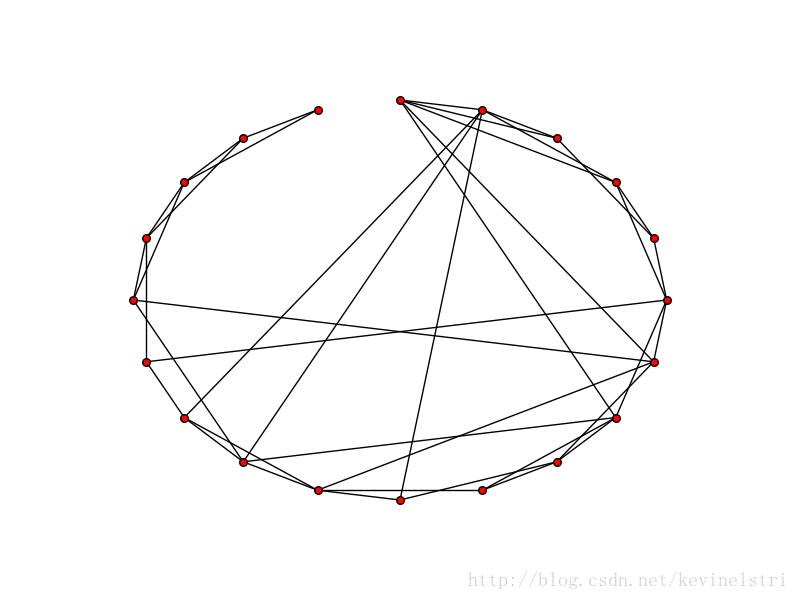
\includegraphics[width=0.6\textwidth]{img/WS.png}
					\caption{WS小世界网络图} 
					\label{img}
				\end{figure}
				
				BA模型:开始有0个节点,每次加入一个节点,并以一定概率(概率和已有节点的度是成正比的,度越大的节点越有可能被连接)与已存在的m个节点相连,直到有n个点。BA模型考虑到现实网络中节点的幂律分布特性,生成无标度网络。
				
				\begin{figure}
					\centering
					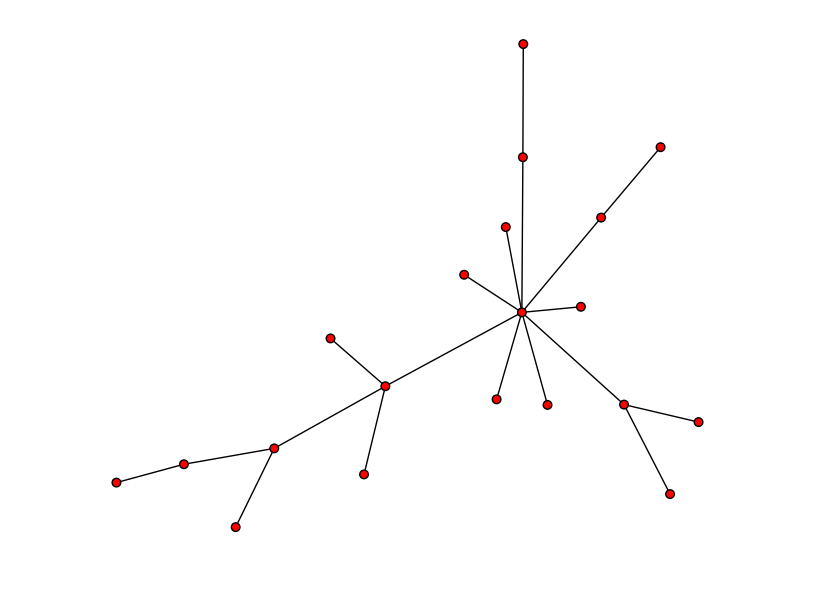
\includegraphics[width=0.6\textwidth]{img/BA.png}
					\caption{BA无标度网络图} 
					\label{img}
				\end{figure}
			
			\subsubsection{虚拟社区及发现技术}
			
				虚拟社区基于子图局部性的定义:社区结构是复杂网络节点集合的若干子集,每个子集内部的节点之间的连接相对非常紧密,而不同子集节点之间的连边相对稀疏。
			
				在社交网络中发现虚拟社区有助于理解网络拓扑结构特点,揭示复杂系统内在功能特性,理解社区内个体关系。为信息检索、信息推荐、信息传播控制和公共事件管控提供有力支撑。虚拟社区发现存在着许多经典的算法,这些算法用于挖掘不同规模的虚拟社区,算法在追求高精度的同时力求提高效率(降低时间复杂度)。
			
			\subsubsection{虚拟社区演化分析}
				
				在线社交网络中存在着大量显性或者隐性的虚拟社区结构,这些虚拟社区结构并不是永恒不变的,随着事件变化,社区结构也在不断演变。分析动态的虚拟社区结构演化有助于理解整个社交网络的演化过程,所以有着重要的研究价值。
				
				虚拟社区涌现即在社交网络中虚拟社区从无到有的过程,其最重要的特征是网络聚集现象。
				
				在线社交网络虚拟社区演化过程非常复杂,影响因素很多。如何挖掘虚拟社区演化中的关键性因素成为社交网络研究中一个重要而有挑战性的课题, 用户个体的累积效应、结构多样性和结构平衡性三个基本因素对虚拟社区演化都存在影响。
		
		\subsection{社交网络群体行为形成与互动规律}
		
			\subsubsection{用户行为分析}
				
				社交网络用户行为是用户对自身需求,社会影响和社交网络技术进行综合评估的基础上做出的使用社交网络服务的意愿,以及由此引起的各种使用活动的总和。用户行为是在线社交网络研究的重要内容。现有研究主要基于如下两种思路展开,一是将在线社交网络作为一种特定的信息技术,研究用户对在线社交网络技术的采纳行为、拒绝行为和用户忠诚;二是将在线社交网络视为提供各种服务和应用的平台,研究用户使用各种服务和应用所表现出的特征与规律。
			
			
			\subsubsection{社交网络情感分析}
			
				随着互联网技术的迅速发展,网络已经成为人们获取信息,发表意见的主要途径,根据文本内容,我们可以将网络中的文本分为两种,一种是客观描述信息,主要针对事件、产品等进行客观描述,另一种是主观性信息,主要产生与用户对人物、事件、产品进行客观性描述;另一种是主观性信息,主要产生于用户对人物、事件、产品等的评价信息。主观性信息表达了人们的各种情感色彩和情感倾向,如“支持”、“反对”、“中立”等。
				
				情感分析,在此等同于意见挖掘,是针对主观性信息进行分析、处理和归纳过程。情感分析最初起源于自然语言处理领域,主要从语法语义规则方面对文本的情感倾向性进行研判。随着社交网络的兴起与发展,情感分析逐渐涉及多个研究领域,如文本挖掘、Web 数据挖掘等,并延伸至管理学及社会科学等学科,并在产品评论、舆情监控、信息预测等多个领域发挥着重要的作用。
			
			\subsubsection{个体影响力分析}
			
				发现社交网络中的有影响力的个体是社交网络研究中非常重要的研究分支,而且其有着重要的应用价值。例如微博营销,谣言检测,舆情管理等等。
			
		\subsection{社交网络信息传播与演化机理}
		
			\subsubsection{在线社交网络信息检索}
				
				信息检索(Information Retrieval) 是从大规模非结构化数据中获取信息的过程,例如搜索引擎就是典型的信息检索技术的应用。在线社交网络数据结构有其特殊性,以微博的“话题”(\#话题名称\#)为例,这种新型的信息组织方式是传统信息检索研究没有涉及的,所以对社交网络信息的检索成为了一门研究课题。
				
			\subsubsection{社交网络信息传播规律}
				
				信息传播是人们通过符号、信号、传递、接收与反馈信息的活动,是人们彼此交换意见、思想、情感,已达到互相了解和影响的过程。社交网络信息传播是指以社交网络为媒介进行信息传播的过程。研究社交网络信息传播的规律,有助于我们加深对社交系统的认识,理解社交现象。也有助于模式发现,大影响力节点识别和个性化推荐。下面主要介绍几种社交网络信息传播模型。
			
			\subsubsection{话题发现与演化}
			
				在话题发现和演化的大部分研究中,话题是指一个引起关注的事件或活动,及其所有相关事件和活动。其中,事件或者活动是指在一个特定的时间和地点,发生的一些事情。社交网络语料库中的数据和传统话题发现语料库的数据区别较大,所以我们必须使用新的方法或对传统方法进行改进来适应社交网络数据特点。
				
				一般社交网络例如 Twitter 的数据有以下特点:数据规模大、内容简短、噪声多、数据特征丰富等。下面介绍几种主要的话题发现和演化模型。
				
			\subsubsection{影响力最大化}
			
				影响力最大化是在社交网络中选定信息初始传播用户,使得信息的传播范围能达到最大,即影响力最大。影响力最大化算法的目的就是找出一定数量的用户作为影响力传播的初始节点。对影响力最大化的问题的建模是基于社交网络信息传播模型的。其中最经典的模型是线性阈值和独立级联模型。
				
				影响力最大化算法被证明为 NP-hard问题,下面主要介绍两种典型的影响力最大化算法。
				
				\begin{itemize}
					\item 贪心算法:从单个节点开始,计算每选一个新节点作为初始节点对每个节点带来的边际收益,取能造成边际收益最大的点加入初始节点集合。贪心算法的缺点是计算时间成本较大,但是计算精度较高。
					\item 启发式算法:不同于贪心算法选择任何一个点作为初始节点开始计算,启发式算法先通过一定策略选取一定数量的初始节点,然后计算其影响力传播。其优点是速度快,缺点是精度低。
				\end{itemize}
		
		\subsection{应用}
			
			\subsubsection{社交推荐}
			
				社交推荐顾名思义是利用社交网络或者结合社交行为的推荐,具体表现为推荐 QQ 好友,微博根据好友关系推荐内容等。在线推荐系统最早被亚马逊用来推荐商品,如今,推荐系统在互联网已无处不在,目前大热的概念“流量分发是互联网第一入口”,支撑这个概念有两点核心,其一是内容,另外就是推荐,今日头条在短短几年间的迅速崛起便是最好的证明。
				
				根据推荐系统推荐原理,社交推荐可定义为一种“协同过滤”推荐,即不依赖于用户的个人行为,而是结合用户的好友关系进行推荐。对于互联网上的每一个用户,通过其社交账户能很快定义这个用户众多特点,再加之社交网络用户数之多,使得利用社交关系的推荐近些年备受关注。
				
			\subsubsection{舆情分析}
			
				舆情分析在互联网出现之前就被广泛应用在政府公共管理,商业竞争情报搜集等领域。在社交媒体出现之前,舆情分析主要是线下的报纸,还有线上门户网站的新闻稿件,这些信息的特点是相对专业准确,而且易于分析和管理;但随着社交媒体出现,舆情事件第一策源地已经不是人民日报新华社这样的大媒体,而是某一个名不见经传的微博用户,一个个人微信公众号。他们的特点是信息非常新鲜,缺点是真实度较低且传播十分迅速,难以控制。所以在社交网络下的舆情分析是一门新的学问。
			
			\subsubsection{隐私保护}
			
				隐私问题在互联网时代已经是老生常谈的问题了。在社交网络中,作为用户,我们可能会留下大量痕迹,这些痕迹有隐性的,也有显性的,好不夸张地,社交服务提供商可以根据你的少量痕迹,挖掘到大量你的个人信息,有些信息是你不愿意别人知道的。
				
				这其中存在一个矛盾,即社交服务提供商处于商业目的想尽可能获取你的个人信息,但是你又担心自己的个人信息被泄露。所以在隐私保护领域,一方面要设计足够安全的机制,技术层面的,法律层面的,在保护个人隐私的前提下最大化商业利益和用户的体验。
			
			\subsubsection{用户画像}
			
				用户画像,这是个营销术语,即通过研究用户的资料和行为,将其划分为不同的类型,进而采取不同的营销策略。传统的用户画像最常用的手段就是调查问卷,订阅过杂志和报纸的读者都知道,会有各种各样的有奖问卷,一方面用来获得对于产品的反馈,另一方面就是对你进行画像通。
				
				在社交网络,用户画像方式变得更多了,除了传统的线下问卷变成在线问卷。我们通过用户的行为,一方面通过统计学方法获得一些用户特征(经典的例子是沃尔玛的“啤酒和尿布”,另一方面通过机器学习进行建模和验证获得意外的收获(参见上面提到的腾讯社交广告文章)。
				
			\subsubsection{谣言检测}
			
				谣言检测算是舆情分析的一部分,谣言的确定对于舆情管理非常重要。早起微博因为充斥着大量谣言,使得新浪微博不得不推出“微博辟谣”官方账号,到如今微博以及有许多自发和官方的辟谣账号,微信公众号也是如此。
				
				传统辟谣方法无非是进行试试检验,用证据说话,随着现在机器学习技术的迅速发展,我们也可以通过信息传播的轨迹,信息内容等维度自动判断消息是否属于谣言,而且判断地越迅速,对于舆情管理的意义就越大。同理,这种技术也被应用在社交网络有害信息识别。
			
			\subsubsection{可视化}
			
				可视化是随着大数据一起成为热门话题的。因为人类对于图像信息的理解速度要大于文字信息数百倍,所以讲一些数据可视化有助于人们更生动地理解某一结论或现象。当然不是所有数据都适合可视化,在社交网络中,我们最常见的有信息传播轨迹还有词云图等。
				
		\subsection{社区发现算法}
			
			社区发现:在图中发现n个社区,同一个社区内的连接紧密,而社区间的连接非常稀疏。
			
			\subsubsection{GN算法}
			
				边介数(betweenness):网络中经过该边的最短路径占所有最短路径的比例。
				
				算法步骤如下:
				\begin{itemize}
					\item 计算网络中所有边的介数
					\item 找到介数最高的边,并将它从网络中移除 
					\item 重复以上步骤,直到每个节点就是一个社区为止
				\end{itemize}
				
				\begin{figure}[htbp]
					\centering
					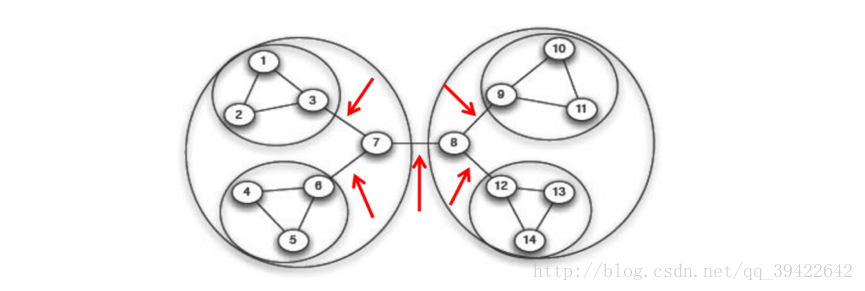
\includegraphics[width=0.8\textwidth]{img/GN.png}
				\end{figure}
			
			\subsubsection{Louvain算法}
			
				Louvain算法是基于模块度的算法,其优化目标就是最大化整个社区网络结构的模块度。
				
				模块度:物理含义是社区内节点的连边数与随机情况下节点的连边数之差,它可以衡量一个社区紧密程度的度量。
				
				\begin{figure}[htbp]
					\centering
					
\includegraphics[width=0.8\textwidth]{img/Louvain.png}
				\end{figure}
				
				算法步骤如下:
				\begin{itemize}
					\item 不断遍历网络中的节点,尝试把单个节点加入能使模块度提升最大的社区,直到所有节点不再改变 
					\item 将第一阶段形成的一个个小的社区并为一个节点,重新构造网络。(边的权重为两个节点内所有原始节点的边权重之和)
					\item 重复以上两步
				\end{itemize}
			
			\subsubsection{LPA算法}
				
				算法步骤如下:
				\begin{itemize}
					\item 初始化每个节点,并赋予唯一标签 
					\item 根据邻居节点最常见的标签更新每个节点的标签 
					\item 最终收敛后标签一致的节点属于同一社区
				\end{itemize}
			
			
			
				
\end{document}